\documentclass[../thesis.tex]{subfiles}
\begin{document}
\chapter{Evaluation Methodologies}
\label{ch:experiments}

There were a myriad of analyses we performed in order to test the efficacy of an Ngram-based engine as described in the previous section. This section looks at how our model responds to some of the challenges we mentioned in Section 1.3 and discusses the interesting results produced. Some of the main questions that we hoped to answer were as follows: 
\begin{itemize}
  \item How well did our placeholders perform?
  \item How does the model perform for smaller datasets?
  \item Does training separate models for different roles improve our accuracies?
\end{itemize}

 We first describe our data, and then analyze the general trend we observed when implementing placeholders. Next, we outline how our analyses show that across both dimensions of time and length, the NLP algorithm is resistant to data scarcity. Furthermore, we showed how breaking up the configurations by router roles gave us unexpected results.

\section{Configuration Data}

We applied our framework to Cisco configurations of core, border, and distribution routers from three large university networks (Table~\ref{tab:datasets}). Figure ~\ref{fig:configs} shows us the distribution by size for configurations from all universities combined. Additionally, we were also able to get extensive data from University A's version control histories. This allowed us to perform some tests based on snapshots sampled across time. We used monthly time intervals for such tests.

\begin{figure}[H]
	\centering
	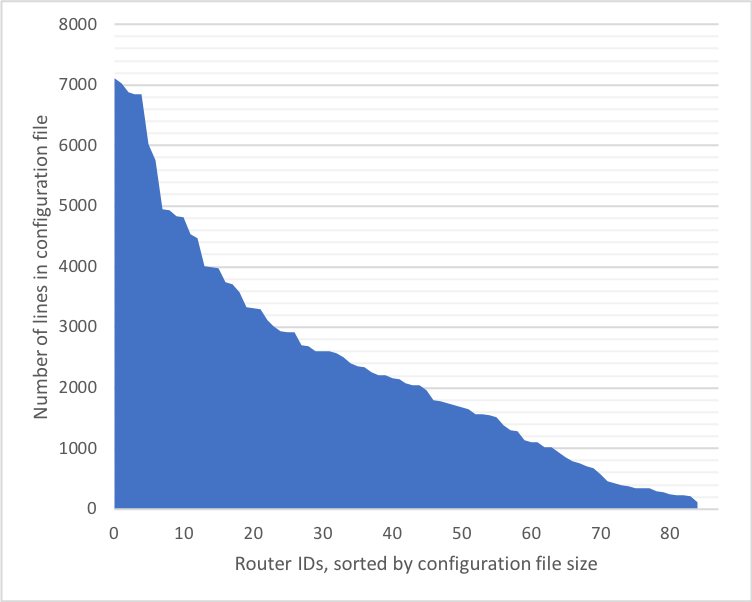
\includegraphics[width=5in]{config_sizes.png}
	\caption{Our data has a good mixture of long and short configurations}
	\label{fig:configs}
\end{figure}

\begin{table}
    \small \centering
    \begin{tabular}{ | c | c | c | c |}
    \hline
        \textbf{Univ.} & \textbf{No. of Configs} & \textbf{Total Lines} & \textbf{Avg Lines} \\ 
    \hline
    A & 35 & 73K & 2.1K \\ 
    B & 26 & 61K & 2.3K \\ 
    C & 24 & 67K & 2.8K \\ 
    \hline
    \end{tabular}
    \caption{Configurations used in our evaluation}
    \vspace{-1em}
    \label{tab:datasets}
\end{table}


\section{Testing Methodology}

To test the accuracy of our model, we perform Leave One Out (LOO) Cross Validation. This form of cross validation involves using one observation as the validation set and the remaining observations as the training set. This is repeated for all combinations of training sets, allowing every observation to act as a validation set. For our analyses an observation could be one set of configurations or just one device configuration depending on the test. For example, for our analyses on length of histories, a validation set is comprised of all device configurations for a given month whereas for an analysis on the number of devices, the validation set is the configuration of one routing device.\\

For a single test, we "walk through" rebuilding the validation set token-by-token, starting from the first keyword. For every line we do not predict the first token but invoke the model for every subsequent token. Figure 5.2 shows us what this test conceptually looks like. On the left handside we have a configuration that is being built using the model and on the right the complete original configuration. Consider the line pointed to by the red arrow. We assume that the first keyword ("ip") is given to us. We then use the model to generate three suggestions
\footnote{The code completion papers we read considered a prediction to be correct if it appeared within the top three to five suggestions. Accurately predicting the correct token within one suggestion every time can be extremely difficult for any code completion system, which is why developers give themselves some leeway when assessing a model's accuracy.}
for the next token and check against the original configuration see whether the correct token ("address") was within this list of suggestions. The next step would be to consider both "ip" and "address" to generate suggestions for the third token. As we are using trigrams, we do not consider more than two previous tokens at a time. We use the ratio of the number of correct predictions to the number of model invocations as a measure of the model's accuracy.\\

\begin{figure}[H]
	\centering
	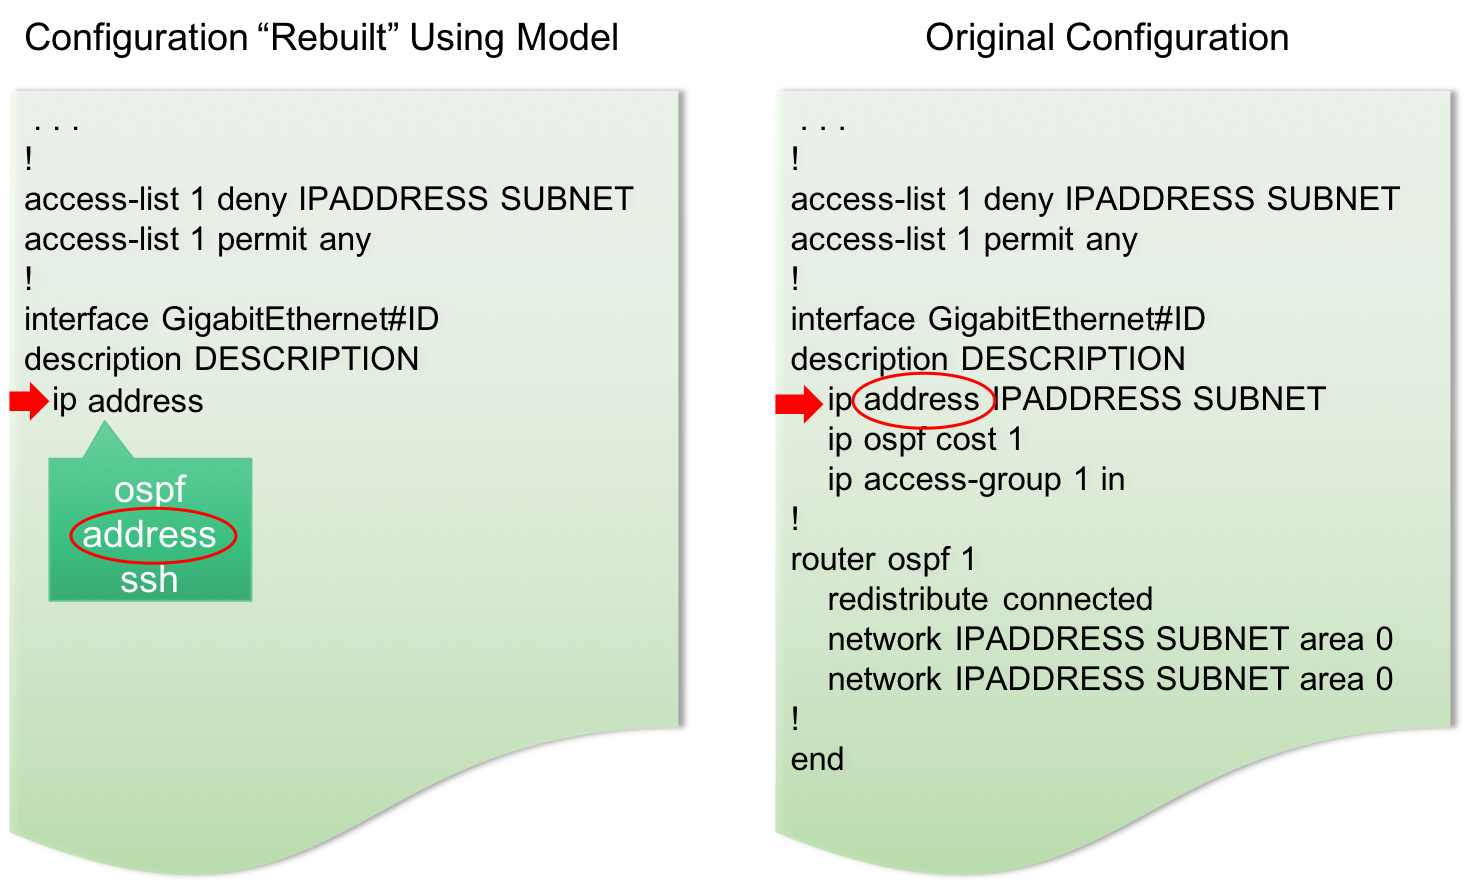
\includegraphics[width=4.2in]{validation_example.png}
	\caption{A visualization of how a validation test is carried out}
\end{figure}
\end{document}
